\documentclass{standalone}
\usepackage{tikz}

\begin{document}
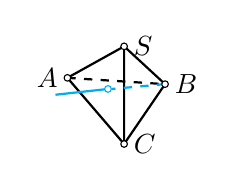
\begin{tikzpicture}[scale=0.4]
\draw[thick] (-1.8,0.6) -- (0,1.6) -- (0,-1.5) -- cycle;
\draw[thick] (0,1.6) -- (1.3,0.4) -- (0,-1.5);
\draw[thick, dashed] (-1.8,0.6) -- (1.3,0.4);

\draw[thick, cyan] (-0.5132,0.247) -- (-2.1795,0.0633) ;
%\draw[thick, cyan, dotted] (1.839,0.4928) -- (-0.396,0.247) ;
\draw[thick, cyan, dashed] (1.3,0.4) -- (-0.396,0.247) ;
\draw[cyan,fill=white] (-0.5132,0.247) circle (3pt);

\draw[fill=white] (-1.8,0.6) circle (3pt) node[left] {$A$};
\draw[fill=white] (0,-1.5) circle (3pt) node[right] {$C$};
\draw[fill=white] (1.3,0.4) circle (3pt) node[right] {$B$};
\draw[fill=white] (0,1.6) circle (3pt) node[right] {$S$};
  
\end{tikzpicture}
\end{document}
